\documentclass{scrartcl}
\usepackage{graphicx}
\usepackage[latin1]{inputenc}
\begin{document}

A free open source crowd simulator

\section{Introduction}

Brainiac is a free and open source tool for generating crowds.
A crowd consists of many agents who respond individually to each other and make decisions about their future behavior.
Brainiac is completely based on open source technology.

\begin{figure}[h]
\centering
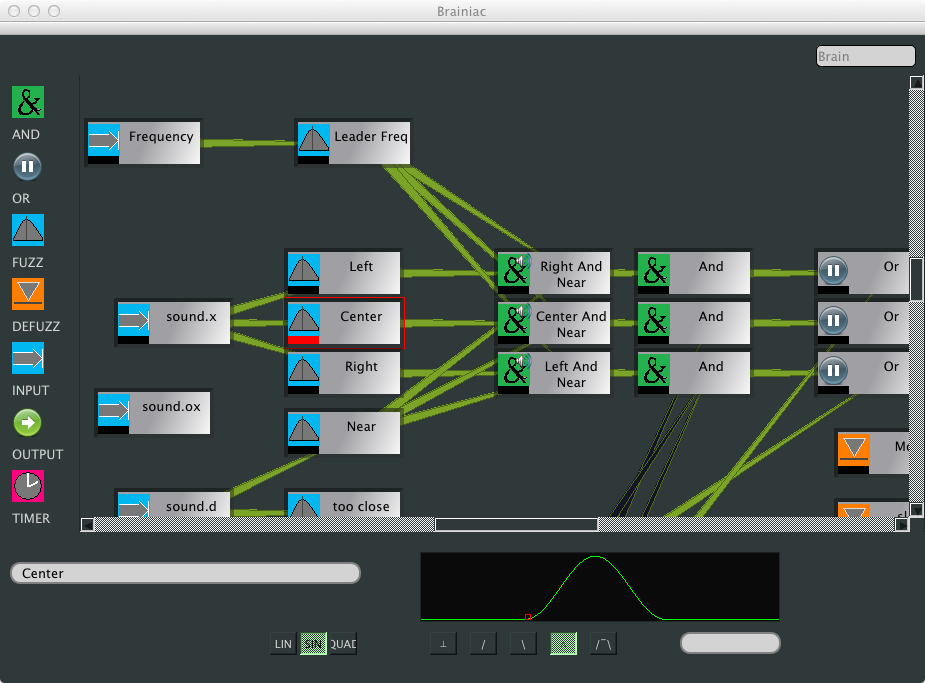
\includegraphics[width=0.8\textwidth]{pics/BrainExampleBig.png}
\caption{Brain of a simple agent}
\end{figure}


\section{Basics}
\subsection{Fuzzy Logic}
Brainiac uses \textit{fuzzy logic} to model a brain of an agent.
\subsection{File formats}
  \begin{itemize}
    \item .bvh (motion, skeleton)
    \item .obj (terrain)
    \item .xml (scene definition, agent definition)
  \end{itemize}

\section{Braineditor}
\subsection{Overview}
\subsection{Fuzzy Nodes}
\subsubsection{AND}

\includegraphics{../gui/pics/editor_logo_and.png}
The AND node is the implementation of fuzzy AND logic. There are two modes that can be used to calculate the output value:
\begin{itemize}
\item PROD use the product of all inputs to determine the output value
\item MIN us the minimum input value to determine the output value
\end{itemize}
It is also possible to calculate fuzzy NAND. Use inverted input connections. Their values will be subtracted from 1 before being calculated. This represents the fuzzy NAND rule.
\subsubsection{OR}

\includegraphics{../gui/pics/editor_logo_or.png}
The OR node is the implementation of fuzzy OR logic. There are two modes that can be used to calculate the output value:
\begin{itemize}
\item SUM use the sum of all inputs to determine the output value
\item MAX us the maximum input value to determine the output value
\end{itemize}
It is also possible to calculate fuzzy NOR. Use inverted input connections. Their values will be subtracted from 1 before being calculated. This represents the fuzzy NOR rule.
\subsubsection{FUZZ}

\includegraphics{../gui/pics/editor_logo_fuzz.png}
\subsubsection{DEFUZZ}

\includegraphics{../gui/pics/editor_logo_defuzz.png}
\subsubsection{INPUT}

\includegraphics{../gui/pics/editor_logo_input.png}
\subsubsection{OUTPUT}

\includegraphics{../gui/pics/editor_logo_output.png}
\subsubsection{TIMER}

\includegraphics{../gui/pics/editor_logo_timer.png}
\subsubsection{NOISE}

\includegraphics{../gui/pics/editor_logo_noise.png}

\section{Bodyeditor}

\section{Actioneditor}

\end{document}